% Wie erstellt man den Zeitplan?
% 1. man läd sich den HTML Code von ese.ifsr.de herunter
% 2. man fügt folgendes CSS manuell hinzu und bestaunt das Ergebnis:
%  *{font-size:0.99!important}
%	main {margin:0;padding:0;}
%	.row {margin:0;}
%	 header, footer, .sidebar, .panel, section h2, section p, #barrierfree-heading, #timetable-heading  {display:none;}
%	tr, td  {line-height: 1em;}
%	table tbody tr td div.table-spacer {height: 1rem;!important}
%	#content {padding:0;}
%
%	td.data {width: 20%; background: #FDC412}
% 3. man benutzt z.B. wkhtmltopdf um ein PDF daraus zu erstellen:
% wkhtmltopdf -s A4 --no-print-media-type --margin-left 0 --margin-right 0 --margin-bottom 0 --margin-top 0 ESE\ 2016\ _\ iFSR.html zeitplan.pdf
% 4. ????
% 5. Färdsch


\addchap[Zeitplan der ESE-Woche]{}

%\thispagestyle{empty} %keine Seitenzahl
%\AddToShipoutPicture*{\put(0,0){%
%\parbox[b][\paperheight]{\paperwidth}{%
\vfill
\begin{center}
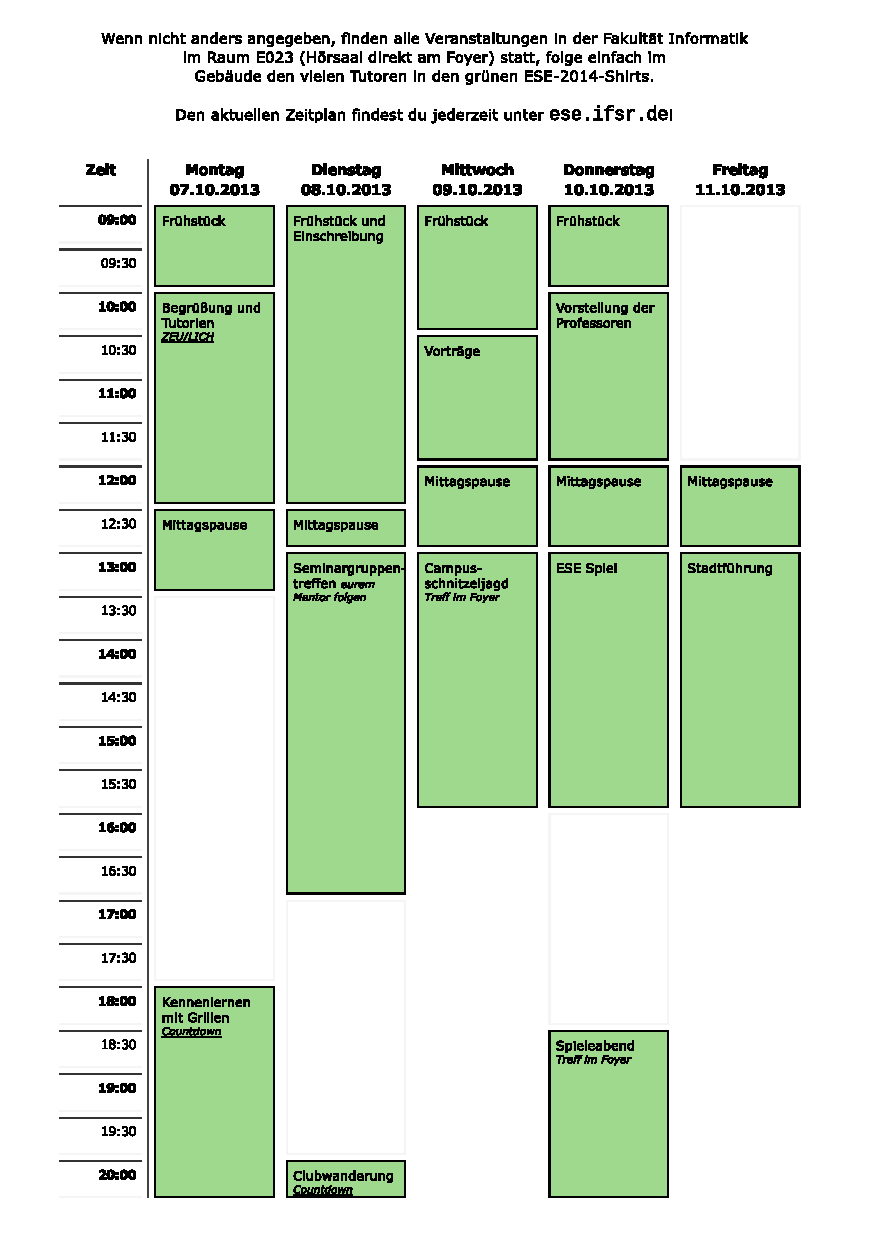
\includegraphics[height=.61\dimen108,keepaspectratio]{img/zeitplan.pdf}%
\vfill

Sofern nicht anders angegeben, finden alle Veranstaltungen im Fakultätsgebäude der Informatik, dem
\textbf{Andreas Pfitzmann Bau (APB)}, im Raum \textbf{E023} (Hörsaal direkt am Foyer) statt.
Folge im Gebäude einfach den vielen Tutoren in den schönen, gelben ESE-2016-Shirts.
Den aktuellen Zeitplan findest du auch jederzeit unter \textbf{ese.ifsr.de} \link{https://ese.ifsr.de/}.

\end{center}
\mbox{}
